% Editable boundary annotations over a mesh-derived PNG; no new figure number.
\begin{tikzpicture}[font=\footnotesize]
  \node[anchor=south west,inner sep=0] (mesh) at (0,0)
    {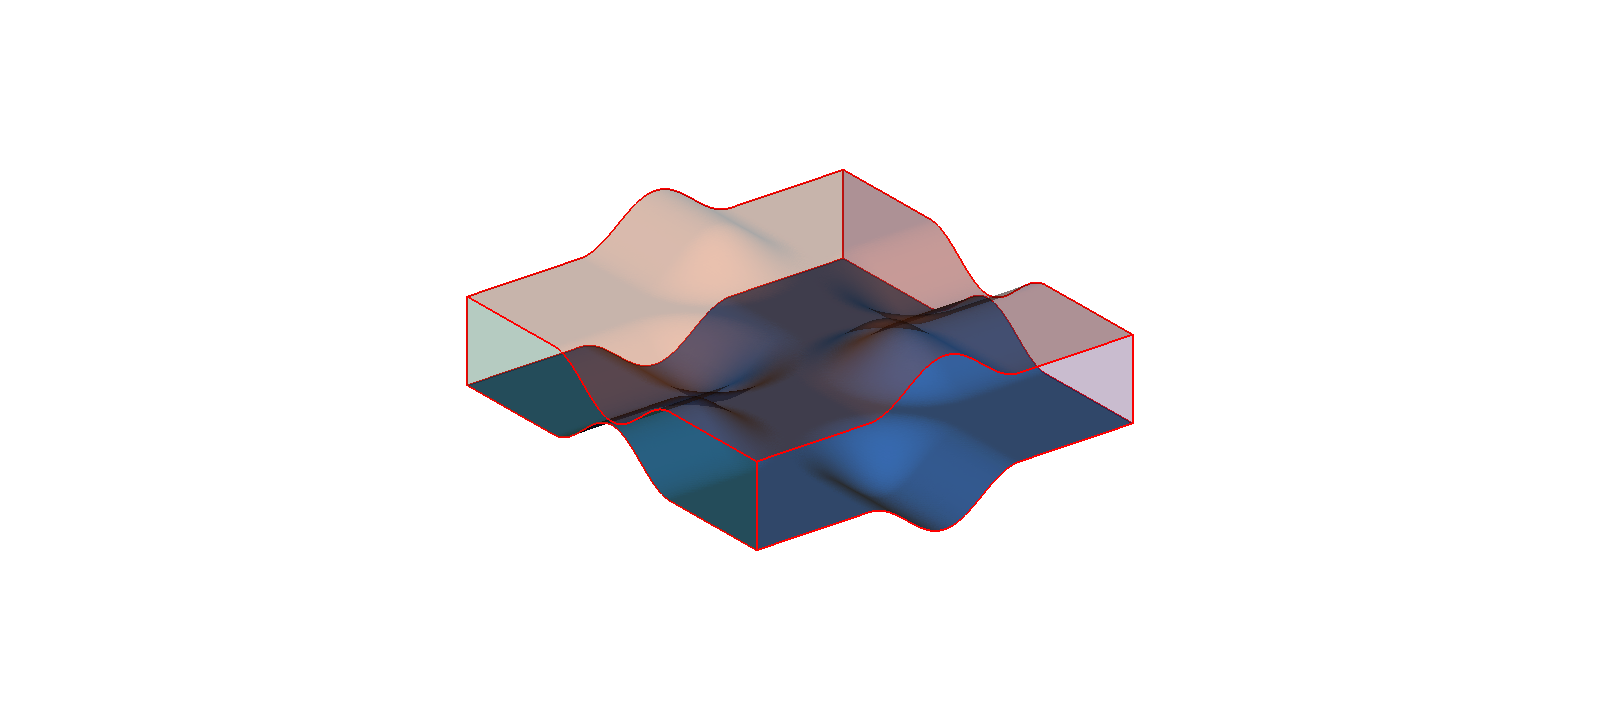
\includegraphics[width=0.96\linewidth]{media/BoundaryMap_CA0.png}};
  \begin{scope}[x={(mesh.south east)},y={(mesh.north west)}]
    \tikzset{labelbox/.style={fill=white,fill opacity=0.95,text opacity=1,align=center,inner sep=2pt},
             pointer/.style={->,line width=0.55pt}}
    \node[anchor=west] at (0.03,0.91) {\textbf{(c)} $\theta_c = 0^o$ boundary map};
    \node[labelbox,text=blue!70!black] (w1) at (0.80,0.17) {\texttt{wall\_1}: lower\\$T_w=333$ K};
    \draw[pointer,blue!70!black] (w1.west) -- (0.53,0.30);
    \node[labelbox,text=orange!70!black] (w2) at (0.66,0.88) {\texttt{wall\_2}: upper\\$T_w=333$ K};
    \draw[pointer,orange!70!black] (w2.south) -- (0.50,0.64);
    \node[labelbox,text=green!40!black] (in) at (0.15,0.41) {\texttt{inlet}\\$x=-12.5$ mm\\$T_{in}=293$ K};
    \draw[pointer,green!40!black] (in.east) -- (0.36,0.44);
    \node[labelbox,text=violet] (out) at (0.84,0.61) {\texttt{outlet}\\$x=+12.5$ mm\\$p_g=0$ Pa};
    \draw[pointer,violet] (out.west) -- (0.65,0.53);
    \node[labelbox] (p1) at (0.39,0.14) {\texttt{span\_top}\\$y=-12.5$ mm};
    \draw[pointer] (p1.north) -- (0.55,0.33);
    \node[labelbox] (p2) at (0.30,0.85) {\texttt{span\_bot}\\$y=+12.5$ mm};
    \draw[pointer] (p2.south) -- (0.45,0.68);
    \node[labelbox] at (0.55,0.48) {Water passage};
    \node[align=center] at (0.53,0.015) {Lateral faces: periodic pair; walls: no-slip};
  \end{scope}
\end{tikzpicture}
